\appendix
\chapter{Genome preprocessing and filtering}




\begin{figure}[H]
	\centering
	\includesvg[width=\textwidth]{asymmetry/spearman_correlation/joinedDatasets/mean_imputed/not_subsampled/filteredSnps/filteredGwas.svg}
	\caption[Effect of 1000G phase3 SNP set filtering on entire hemisphere GWAS]{Entire hemisphere \ac{gwas}, with grayed out the \acp{snp} removed when filtering with 1000G phase3 \ac{snp} set data.}
	\label{fig:1000g_entire_hemisphere}
\end{figure}


\begin{table}[H]
	\centering
	\subfloat[Overview of the entire hemisphere significant, based on the European threshold 5e-8, \ac{snp} filtering.]{
	\scriptsize
	\resizebox{\textwidth}{!}{\begin{tabular}{lcccccc}\toprule
		&\textbf{Chr.} &\textbf{\# Removed} &\textbf{\# Kept} &\textbf{Rem. Percentage} &\textbf{Removed Min. P-value} &\textbf{Kept Min. P-value} \\\midrule
		&1 &5 &1 &83.33\% &4.31e-25 &4.56e-11 \\
		&2 &175 &74 &70.28\% &1.80e-20 &4.30e-18 \\
		&3 &34 &11 &75.56\% &3.48e-15 &1.26e-15 \\
		&7 &48 &6 &88.89\% &1.76e-10 &1.13e-9 \\
		&8 &31 &16 &65.96\% &1.97e-10 &1.80e-10 \\
		&9 &28 &10 &73.68\% &1.40e-25 &1.81e-24 \\
		&12 &79 &20 &79.80\% &1.71e-13 &4.89e-13 \\
		&14 &51 &16 &76.12\% &1.09e-25 &3.58e-28 \\
		&15 &46 &9 &83.64\% &2.09e-50 &3.94e-50 \\
		&16 &467 &56 &89.29\% &3.78e-21 &1.04e-15 \\
		&17 &99 &5 &95.19\% &3.91e-44 &8.20e-31 \\
		&21 &5 &2 &71.43\% &3.01e-9 &7.89e-9 \\\midrule
		\textbf{Total} &125 &1068 &226 &82.53\% & & \\
		\bottomrule
	\end{tabular}}
	\label{tab:1000g_entire_hemisphere}
}
\quad
\subfloat[Partition-chromosome pairs that had the entirety of Bonferroni significant \acp{snp} (P-value<5e-8/31) removed.]{
\scriptsize
\begin{tabular}{lccccc}\toprule
	\textbf{Chr.} &\textbf{Partition} &\textbf{\# Removed} &\textbf{Removed Min. P-value} &\textbf{Kept Min. P-value} \\\midrule
	16 &4 &6 &1.61e-11 &1.67e-8 \\
	17 &4 &40 &4.87e-11 &1.73e-8 \\
	16 &7 &3 &9.24e-16 &2.51e-9 \\
	17 &12 &4 &4.10e-10 &3.38e-9 \\
	16 &14 &4 &1.18e-13 &6.73e-9 \\
	8 &17 &1 &1.54e-9 &1.74e-9 \\
	15 &22 &1 &8.42e-10 &5.65e-9 \\
	16 &28 &2 &4.98e-10 &3.43e-8 \\
	\bottomrule
\end{tabular}
\label{tab:1000g_lost_bonf_chr}
}
\caption{Effect of 1000G Phase3 filtering on meta-analyzed \ac{gwas} scores} 

\end{table}

\chapter{\Acs{gwas} results}


\begin{figure}[H]
	\begin{adjustwidth}{-3 cm}{-2.5 cm}\centering
		\begin{minipage}{0.45\linewidth}
			\subfloat[Spearman correlation assessing mean substitution effect]{
				\scriptsize
				\begin{tabular}{cc}\toprule
					\textbf{Partition} &\textbf{Spearman Correlation} \\\midrule
					1 &0.9996 \\
					2 &0.9997 \\
					3 &0.9989 \\
					4 &0.9997 \\
					5 &0.9997 \\
					6 &0.9994 \\
					7 &0.9997 \\
					8 &0.9994 \\
					9 &0.9997 \\
					10 &0.9997 \\
					11 &0.9996 \\
					12 &0.9996 \\
					13 &0.9997 \\
					14 &0.9997 \\
					15 &0.9997 \\
					16 &0.9996 \\
					17 &0.9997 \\
					18 &0.9997 \\
					19 &0.9997 \\
					20 &0.9995 \\
					21 &0.9997 \\
					22 &0.9997 \\
					23 &0.9997 \\
					24 &0.9997 \\
					25 &0.9997 \\
					26 &0.9996 \\
					27 &0.9997 \\
					28 &0.9996 \\
					29 &0.9996 \\
					30 &0.9996 \\
					31 &0.9997 \\
					\bottomrule
				\end{tabular}
				\label{tab: spearman_no_vs_mean}
			}
		\end{minipage}
		\quad
		\begin{minipage}{0.45\linewidth}
			\centering
			\subfloat[With substitution]{
				\includesvg[width=1\textwidth]{asymmetry/genomeDemo/STAGE00DATA/mean_imputed/not_subsampled/gwas_discovery.svg}
			}
			\par\medskip
			\centering
			\subfloat[Without substitution]{
				\includesvg[width=1\textwidth]{asymmetry/genomeDemo/STAGE00DATA/not_imputed/not_subsampled/gwas_discovery_not_imputed.svg}	
			}
		\end{minipage}
	\end{adjustwidth}
	\caption{Graphs assessing the quantitative (across partitions) and qualitative effect (on the entire hemisphere) of mean \ac{snp} substitution on the discovery dataset \ac{gwas}.}
\end{figure}

\begin{figure}[H]
	\begin{adjustwidth}{-3 cm}{-2.5 cm}\centering
		
		
		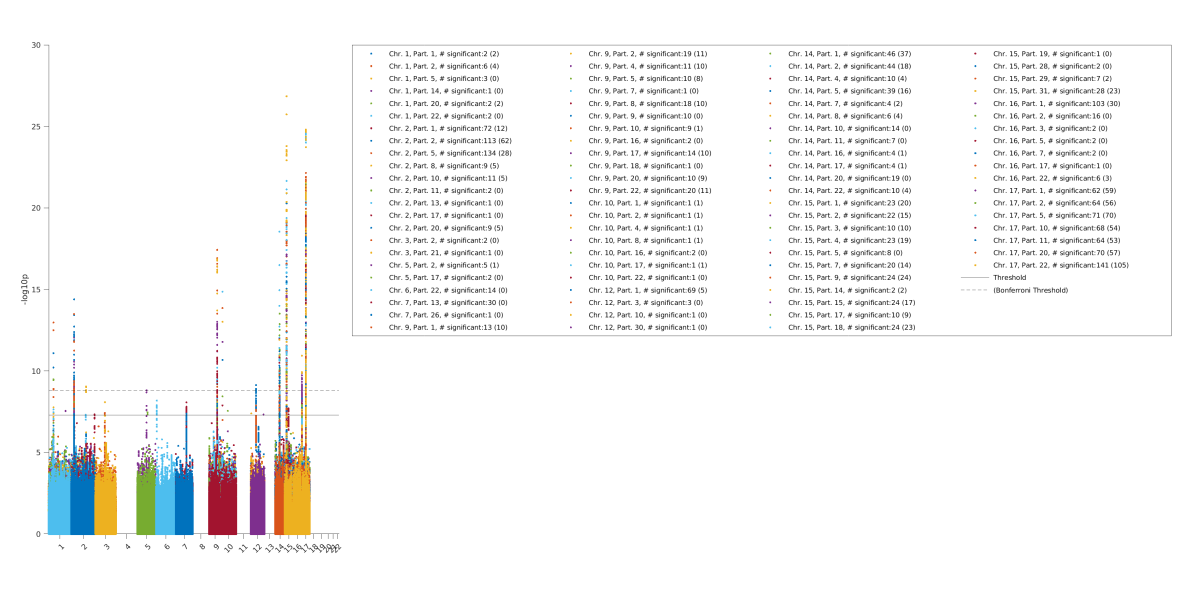
\includegraphics[width=\linewidth]{asymmetry/meta_analysis/joinedDatasets/mean_imputed/not_subsampled/partitions_gwas.pdf}
		\caption[Combined Manhattan plots across different partitions]{Combined Manhattan plots across different partitions, showing the number of significant \acp{snp} below the threshold of 5e-8 and with the Bonferroni correction, inside parentheses.}
		\label{fig:part_manhattan}
		
		
	\end{adjustwidth}
\end{figure}

\begin{adjustwidth}{-3 cm}{-2.5 cm}\centering
	\begin{threeparttable}[!htb]
		\tiny
		\fontsize{4}{7}
		\selectfont
		\setlength\tabcolsep{1.3pt}
		\begin{tabular}{l|c|c|c|c|c|c|c|c|c|c|c|c|c|c|c|c|c|c|c|c|c|c|c|c|c|c|c|c|c|c|c}
			\textbf{Partition} &\textbf{1} &\textbf{2} &\textbf{3} &\textbf{4} &\textbf{5} &\textbf{6} &\textbf{7} &\textbf{8} &\textbf{9} &\textbf{10} &\textbf{11} &\textbf{12} &\textbf{13} &\textbf{14} &\textbf{15} &\textbf{16} &\textbf{17} &\textbf{18} &\textbf{19} &\textbf{20} &\textbf{21} &\textbf{22} &\textbf{23} &\textbf{24} &\textbf{25} &\textbf{26} &\textbf{27} &\textbf{28} &\textbf{29} &\textbf{30} &\textbf{31} \\\hline
			\textbf{Correlation} &0.16 &0.13 &0.14 &0.12 &0.1 &0.1 &0.08 &0.13 &0.06 &0.06 &0.11 &0.1 &0.05 &0.09 &0.04 &0.1 &0.15 &0.05 &0.04 &0.03 &0.04 &0.15 &0.08 &0.16 &0.02 &0.05 &0.02 &0.08 &0.07 &-0.02 &0.01 \\
			\textbf{P-value} &1.2e-11 &1.1e-8 &2.6e-11 &4.3e-7 &7.5e-5 &1.7e-5 &9.6e-4 &5.1e-8 &6.9e-3 &1.8e-2 &4.3e-6 &1.1e-5 &4.0e-2 &2.2e-4 &6.0e-2 &1.5e-5 &1.4e-9 &1.8e-2 &8.4e-2 &1.0e-1 &4.0e-2 &5.1e-10 &2.9e-3 &4.3e-11 &2.6e-1 &2.8e-2 &1.9e-1 &8.2e-4 &5.0e-3 &7.6e-1 &3.7e-1 \\
		\end{tabular}
		\caption{Spearman correlation of the mvGWAS on each partition with the results from \citet{Sha2021}, and the corresponding bootstrap p-values.}\label{tab:otherAsym}
	\end{threeparttable}
\end{adjustwidth}

\chapter{Heritability}
\begin{figure}[H]
	\centering
\includesvg[width=0.5\textwidth]{asymmetry/visualizeHeritabilityOnPheno/joinedDatasets/mean_imputed/not_subsampled/Lambda GC.svg}
\caption[$\lambda_{GC}$ coefficient, as computed by LDSR]{$\lambda_{GC}$ coefficient, as computed by \ac{ldsr}. The observed $\chi^2$ value is close to the expected one at all studied partitions, with their ratio being close to 1.}	
\end{figure}



\chapter{Functional analysis}
\begin{figure}[H]
	\centering
	\subfloat[Cell components]{
		\includegraphics[width=\textwidth]{asymmetry/FUMA gene2func/joinedDatasets/mean_imputed/not_subsampled/partitionsSummary/GO_CC.pdf}
	}
	\quad
	\subfloat[Biological processes]{
		\includegraphics[width=\textwidth]{asymmetry/FUMA gene2func/joinedDatasets/mean_imputed/not_subsampled/partitionsSummary/GO_BP.pdf}
	}
	\quad
	\subfloat[Molecular function]{
		\includegraphics[width=\textwidth]{asymmetry/FUMA gene2func/joinedDatasets/mean_imputed/not_subsampled/partitionsSummary/GO_MF.pdf}
	}
	\caption[GO terms GSEA -log10P values]{\Ac{go} terms enrichment analysis -log10 P-values (the higher value and the darker color, the more significant), as computed by FUMA, with the gene set augmented by GREAT.For all three cases, the entire hemisphere and the four 2nd level partition were assessed, however not all of the tests displayed a significant signal with \ac{go} terms.}
	\label{fig:go}
\end{figure}
\begin{figure}[H]
	\centering
	\subfloat[Cell components]{
		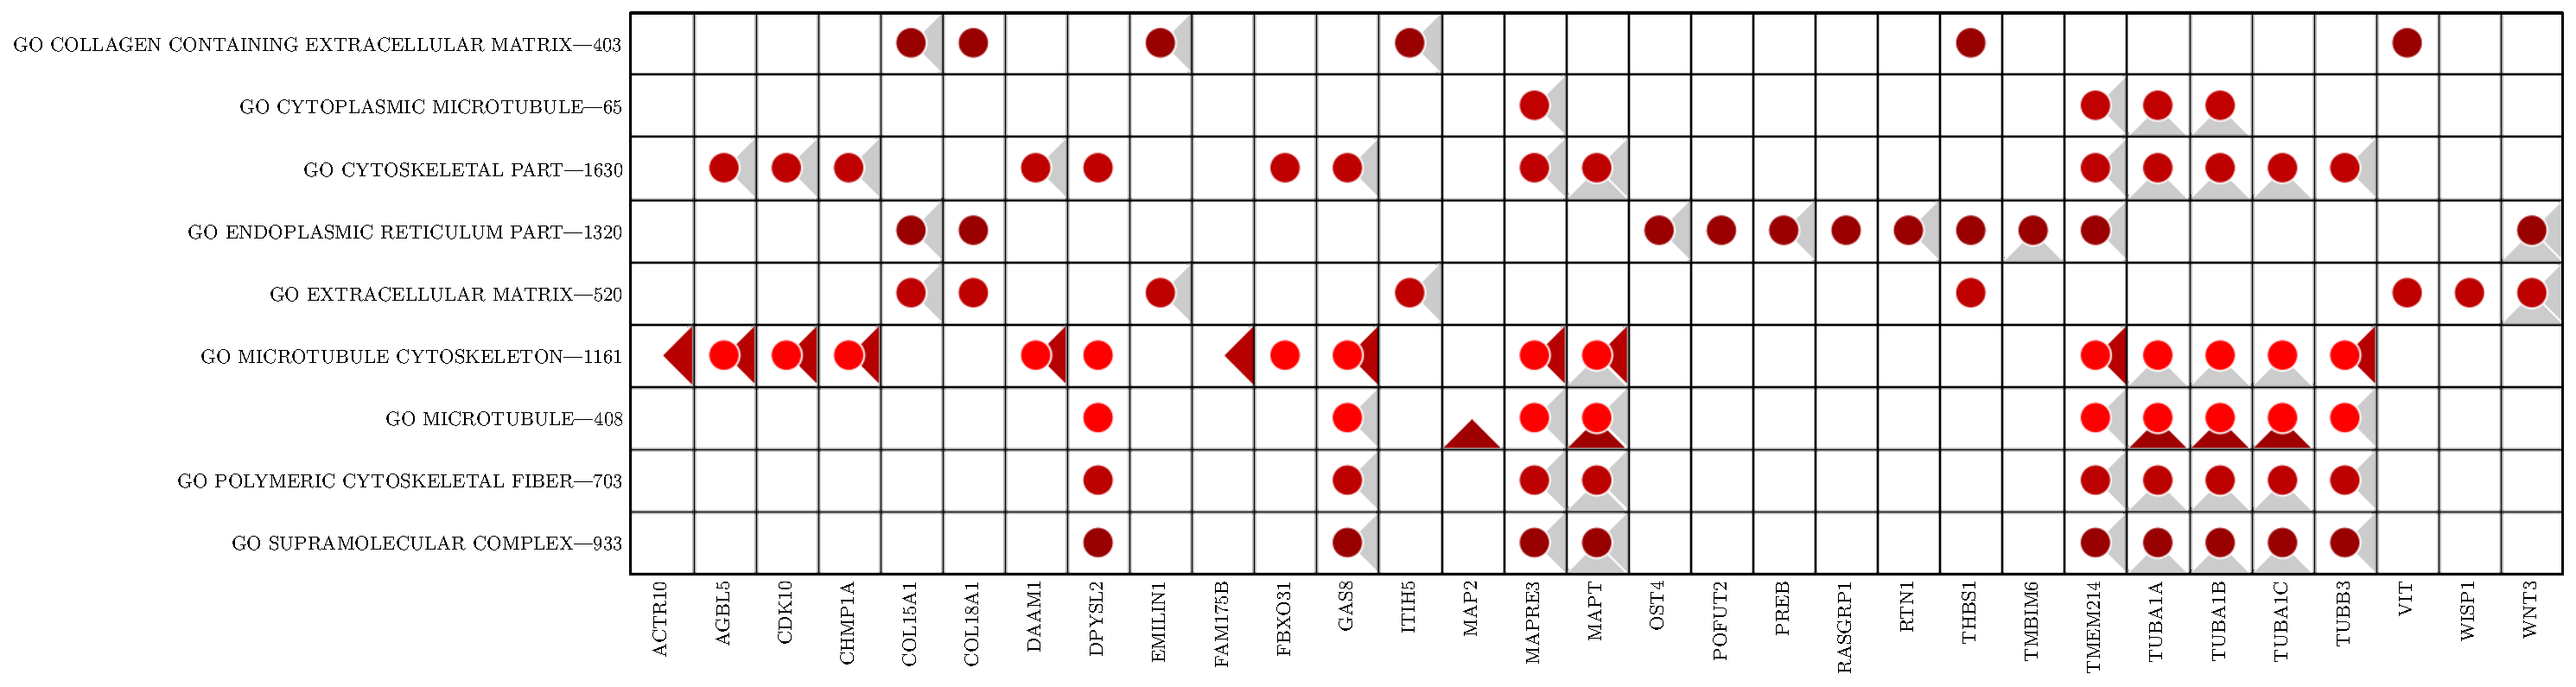
\includegraphics[width=\textwidth]{asymmetry/FUMA gene2func/joinedDatasets/mean_imputed/not_subsampled/partitionsSummary/genes_GO_cc.pdf}
	}
	\quad
	\subfloat[Biological processes]{
		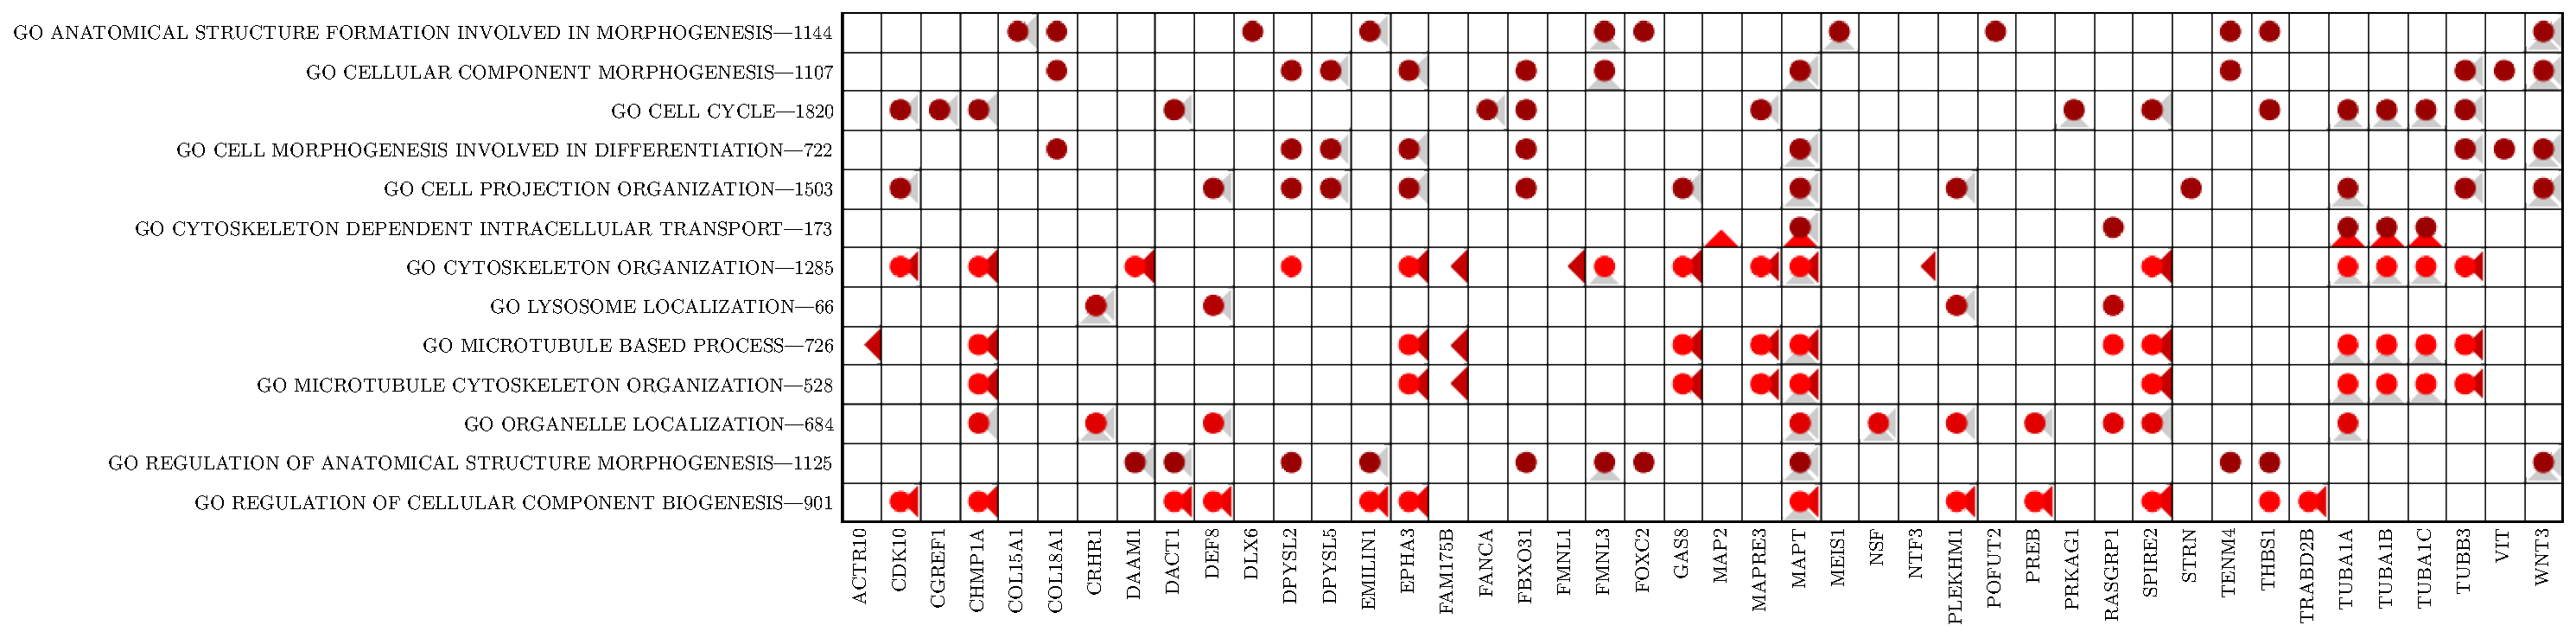
\includegraphics[width=\textwidth]{asymmetry/FUMA gene2func/joinedDatasets/mean_imputed/not_subsampled/partitionsSummary/genes_GO_bp.pdf}
	}
	\quad
	\subfloat[Molecular function]{
		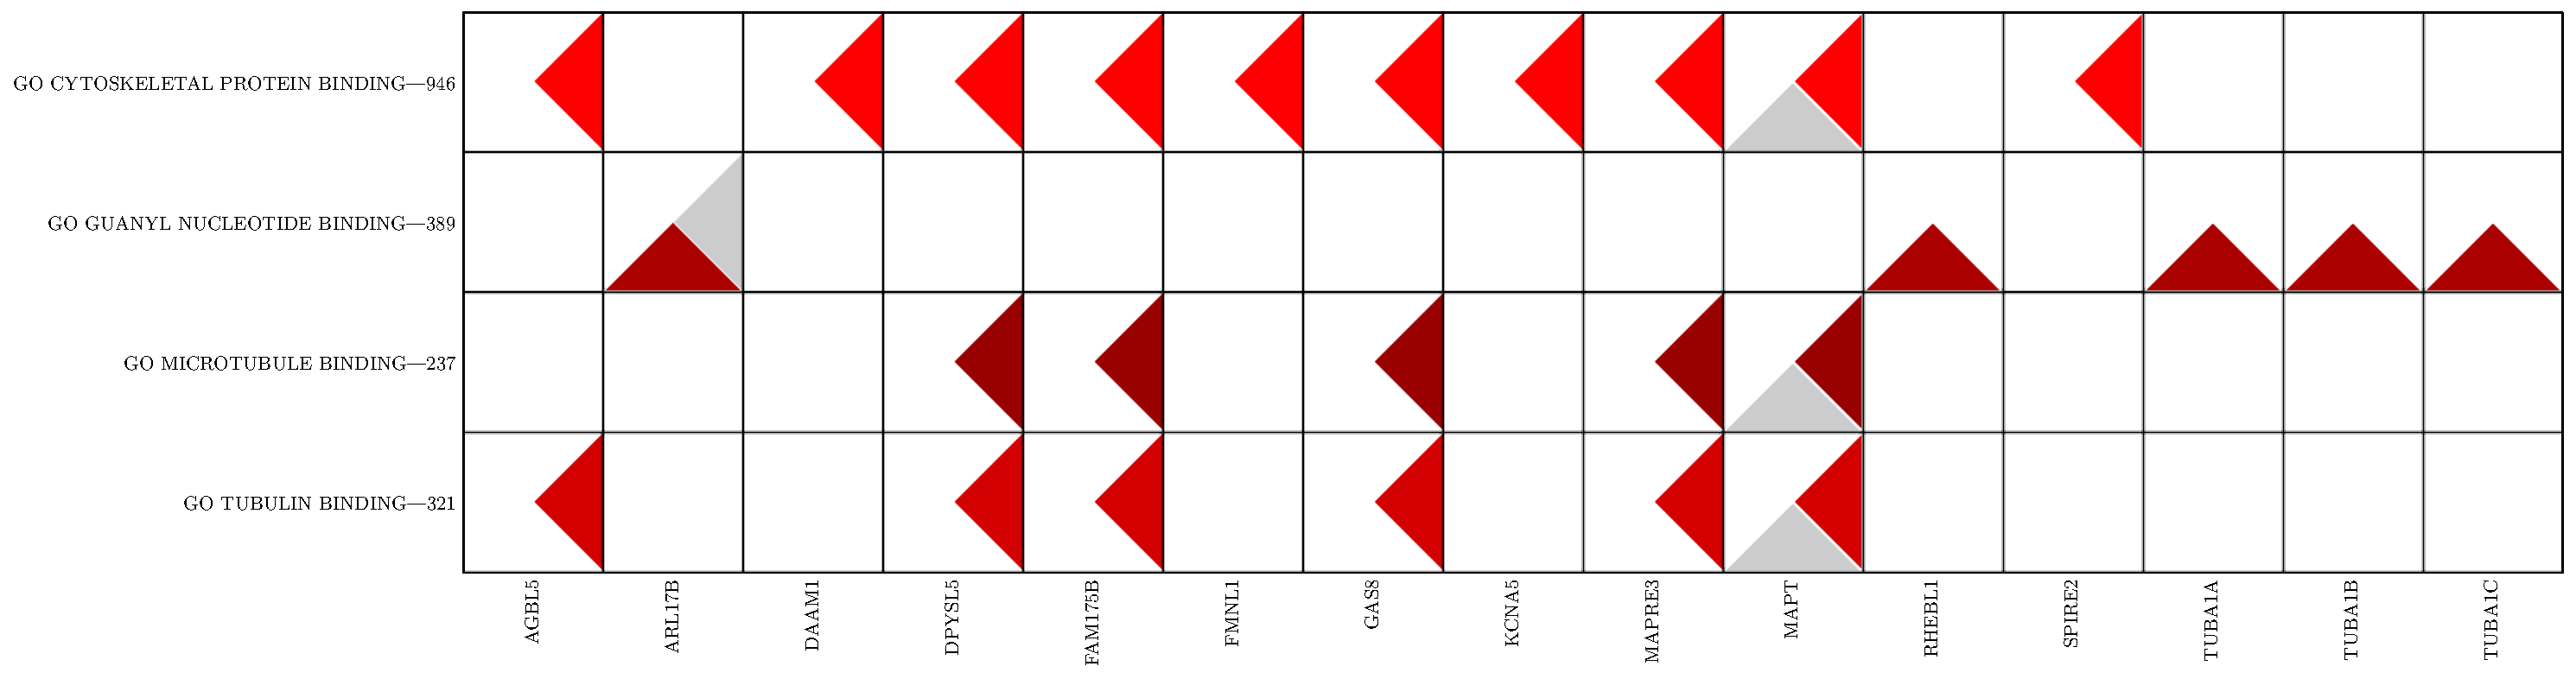
\includegraphics[width=\textwidth]{asymmetry/FUMA gene2func/joinedDatasets/mean_imputed/not_subsampled/partitionsSummary/genes_GO_mf.pdf}
	}
	\caption[GO terms GSEA genes]{\Ac{go} terms enrichment analysis genes (the higher value and the lighter color, the more significant).For all three cases, the entire hemisphere and the four 2nd level partitions (ie. P1 and P4-P7)) were assessed. With gray, genes are shown that, although intersecting with the trait gene set, were not enough for FUMA to identify significant correlation, based on the underlying gene sets sizes ratios. The partition (P) information per cell is coded as follows: circle: P1, north:P4, east:P5, south:P6, west:P7. Next to the name of the category, the total number of related genes is displayed.}
	\label{fig:go_genes}
\end{figure}
\begin{figure}[H]
	\centering
	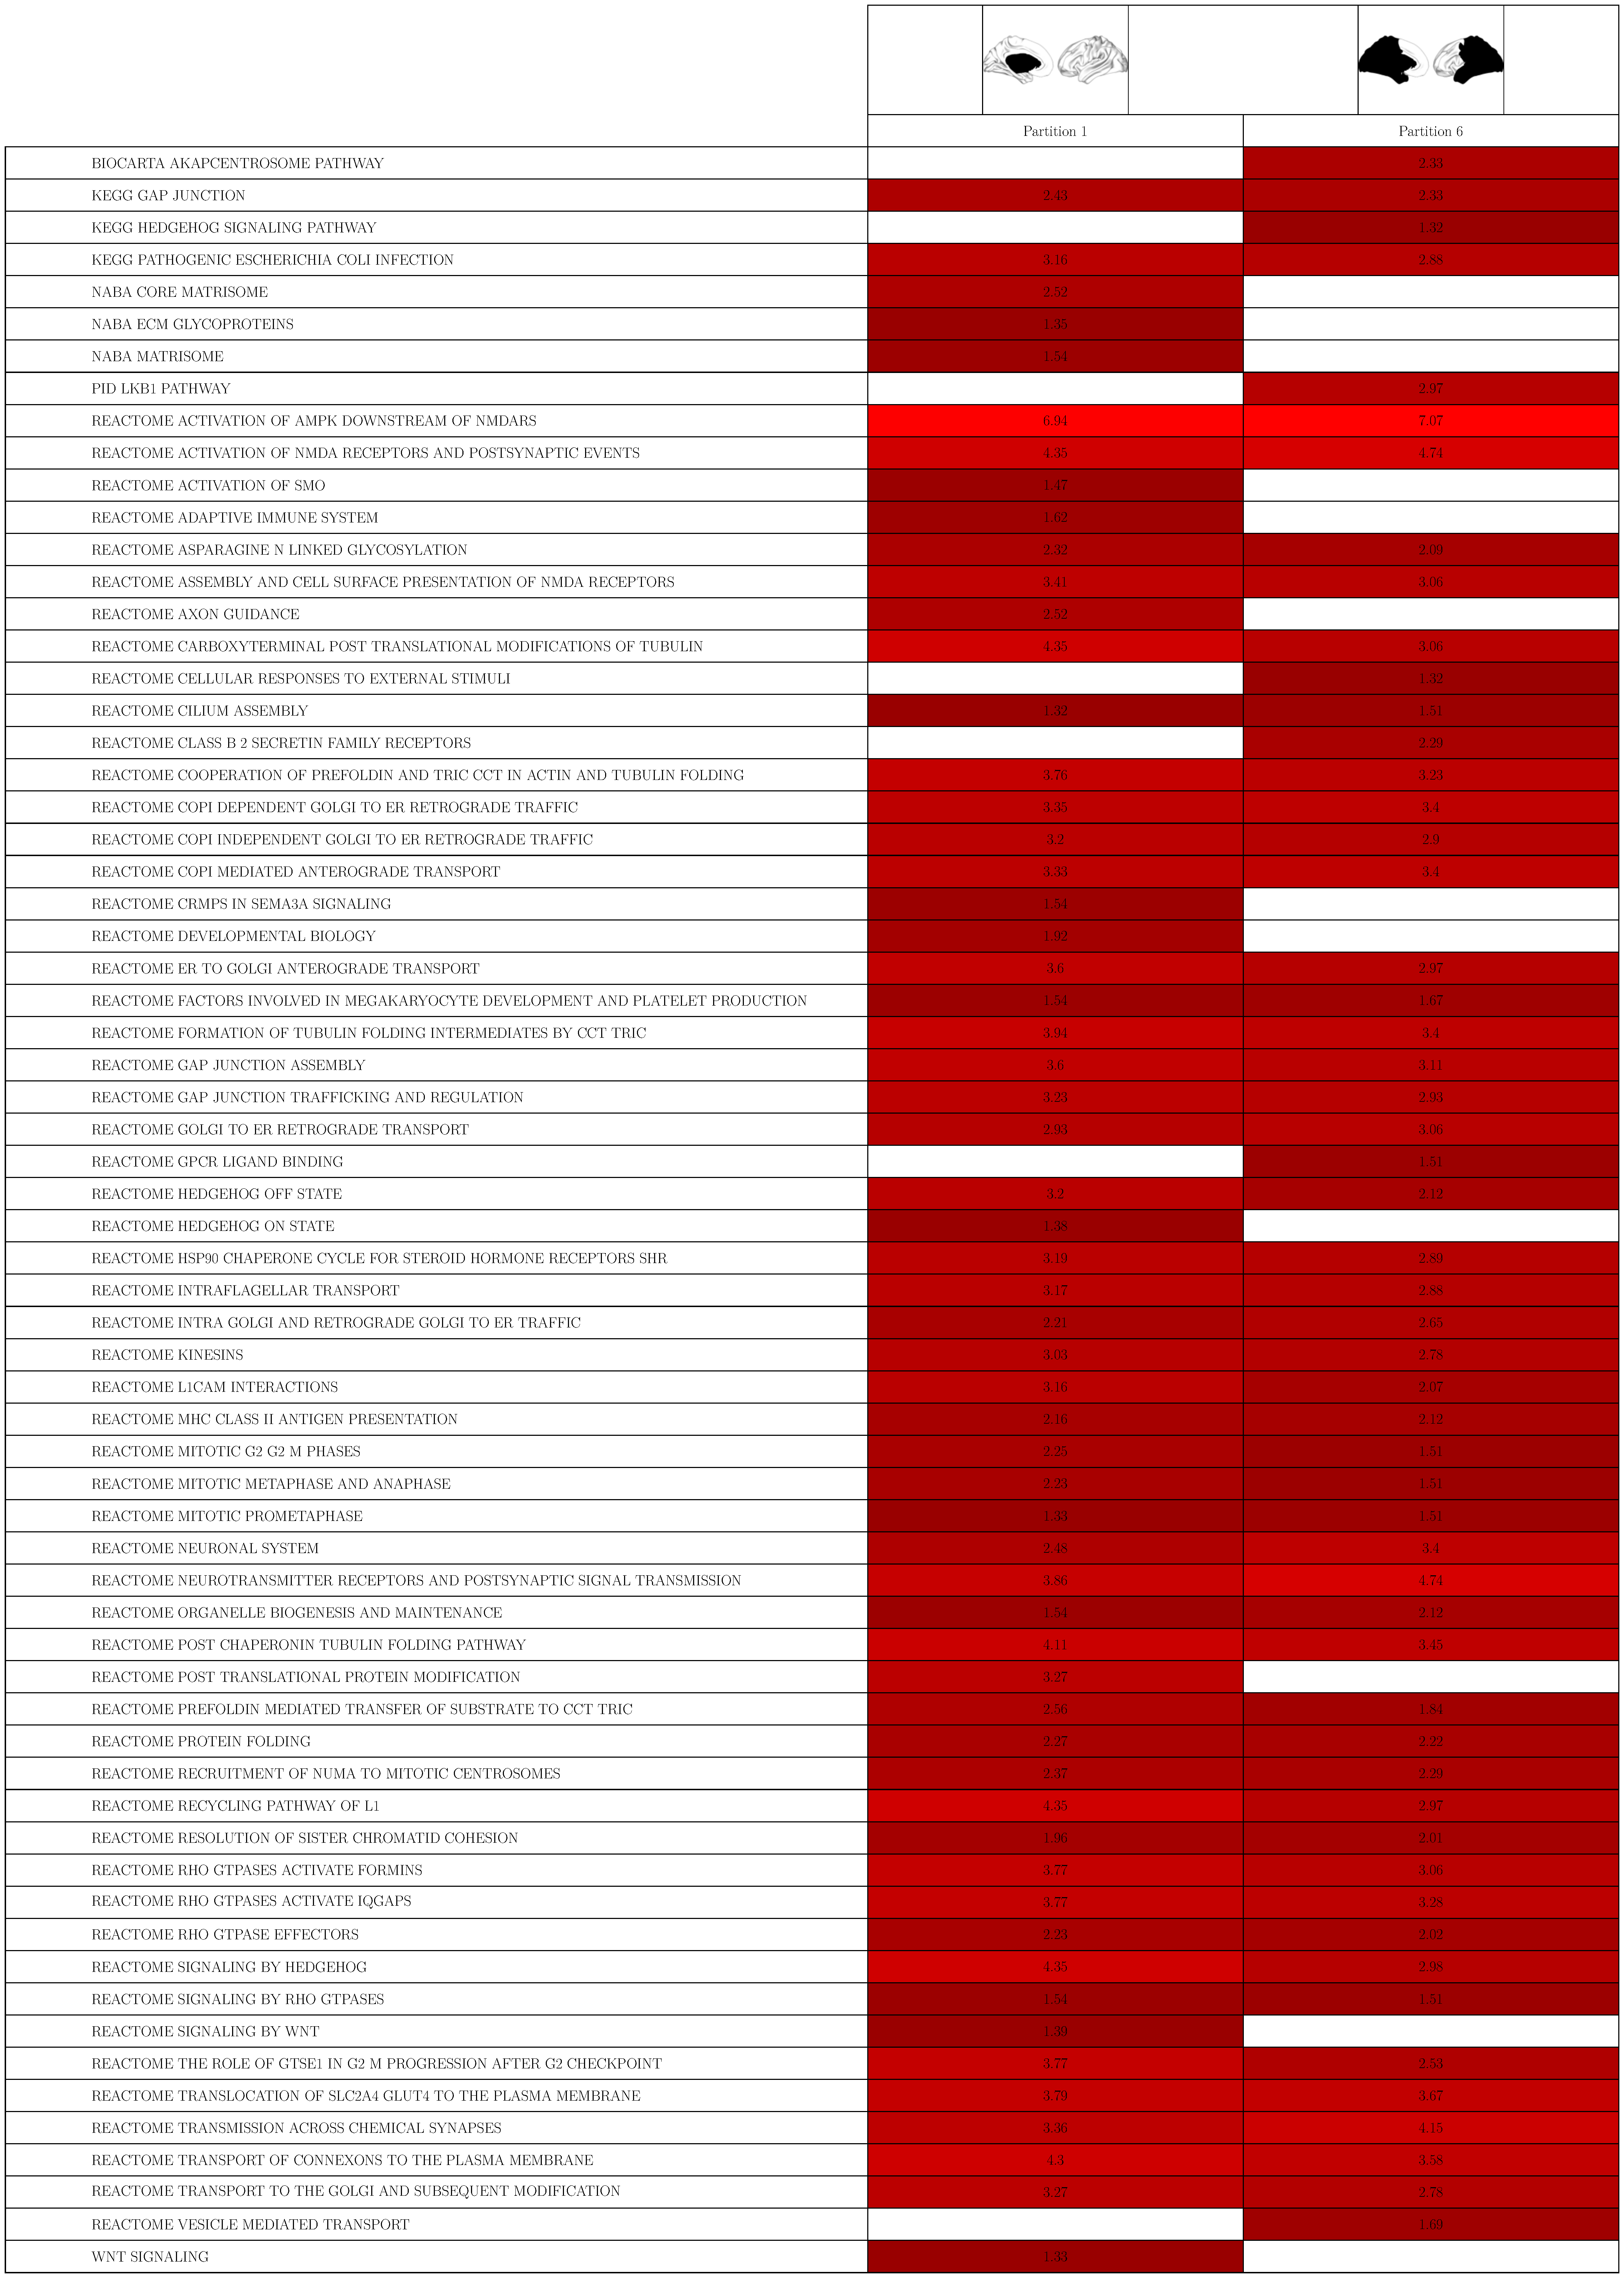
\includegraphics[width=\textwidth]{asymmetry/FUMA gene2func/joinedDatasets/mean_imputed/not_subsampled/partitionsSummary/canonical_pathways.pdf}
	
	\caption[Canonical pathways GSEA -log10P values]{Differential gene set enrichment analysis performed on various canonical pathways reported by KEGG and Reactome, as computed by FUMA. Displayed -log10 P-values have increased lightness the higher the value.}
	\label{fig:can_pathways}
\end{figure}
\begin{adjustwidth}{-3cm}{-3cm}
\begin{figure}[H]
	\centering
	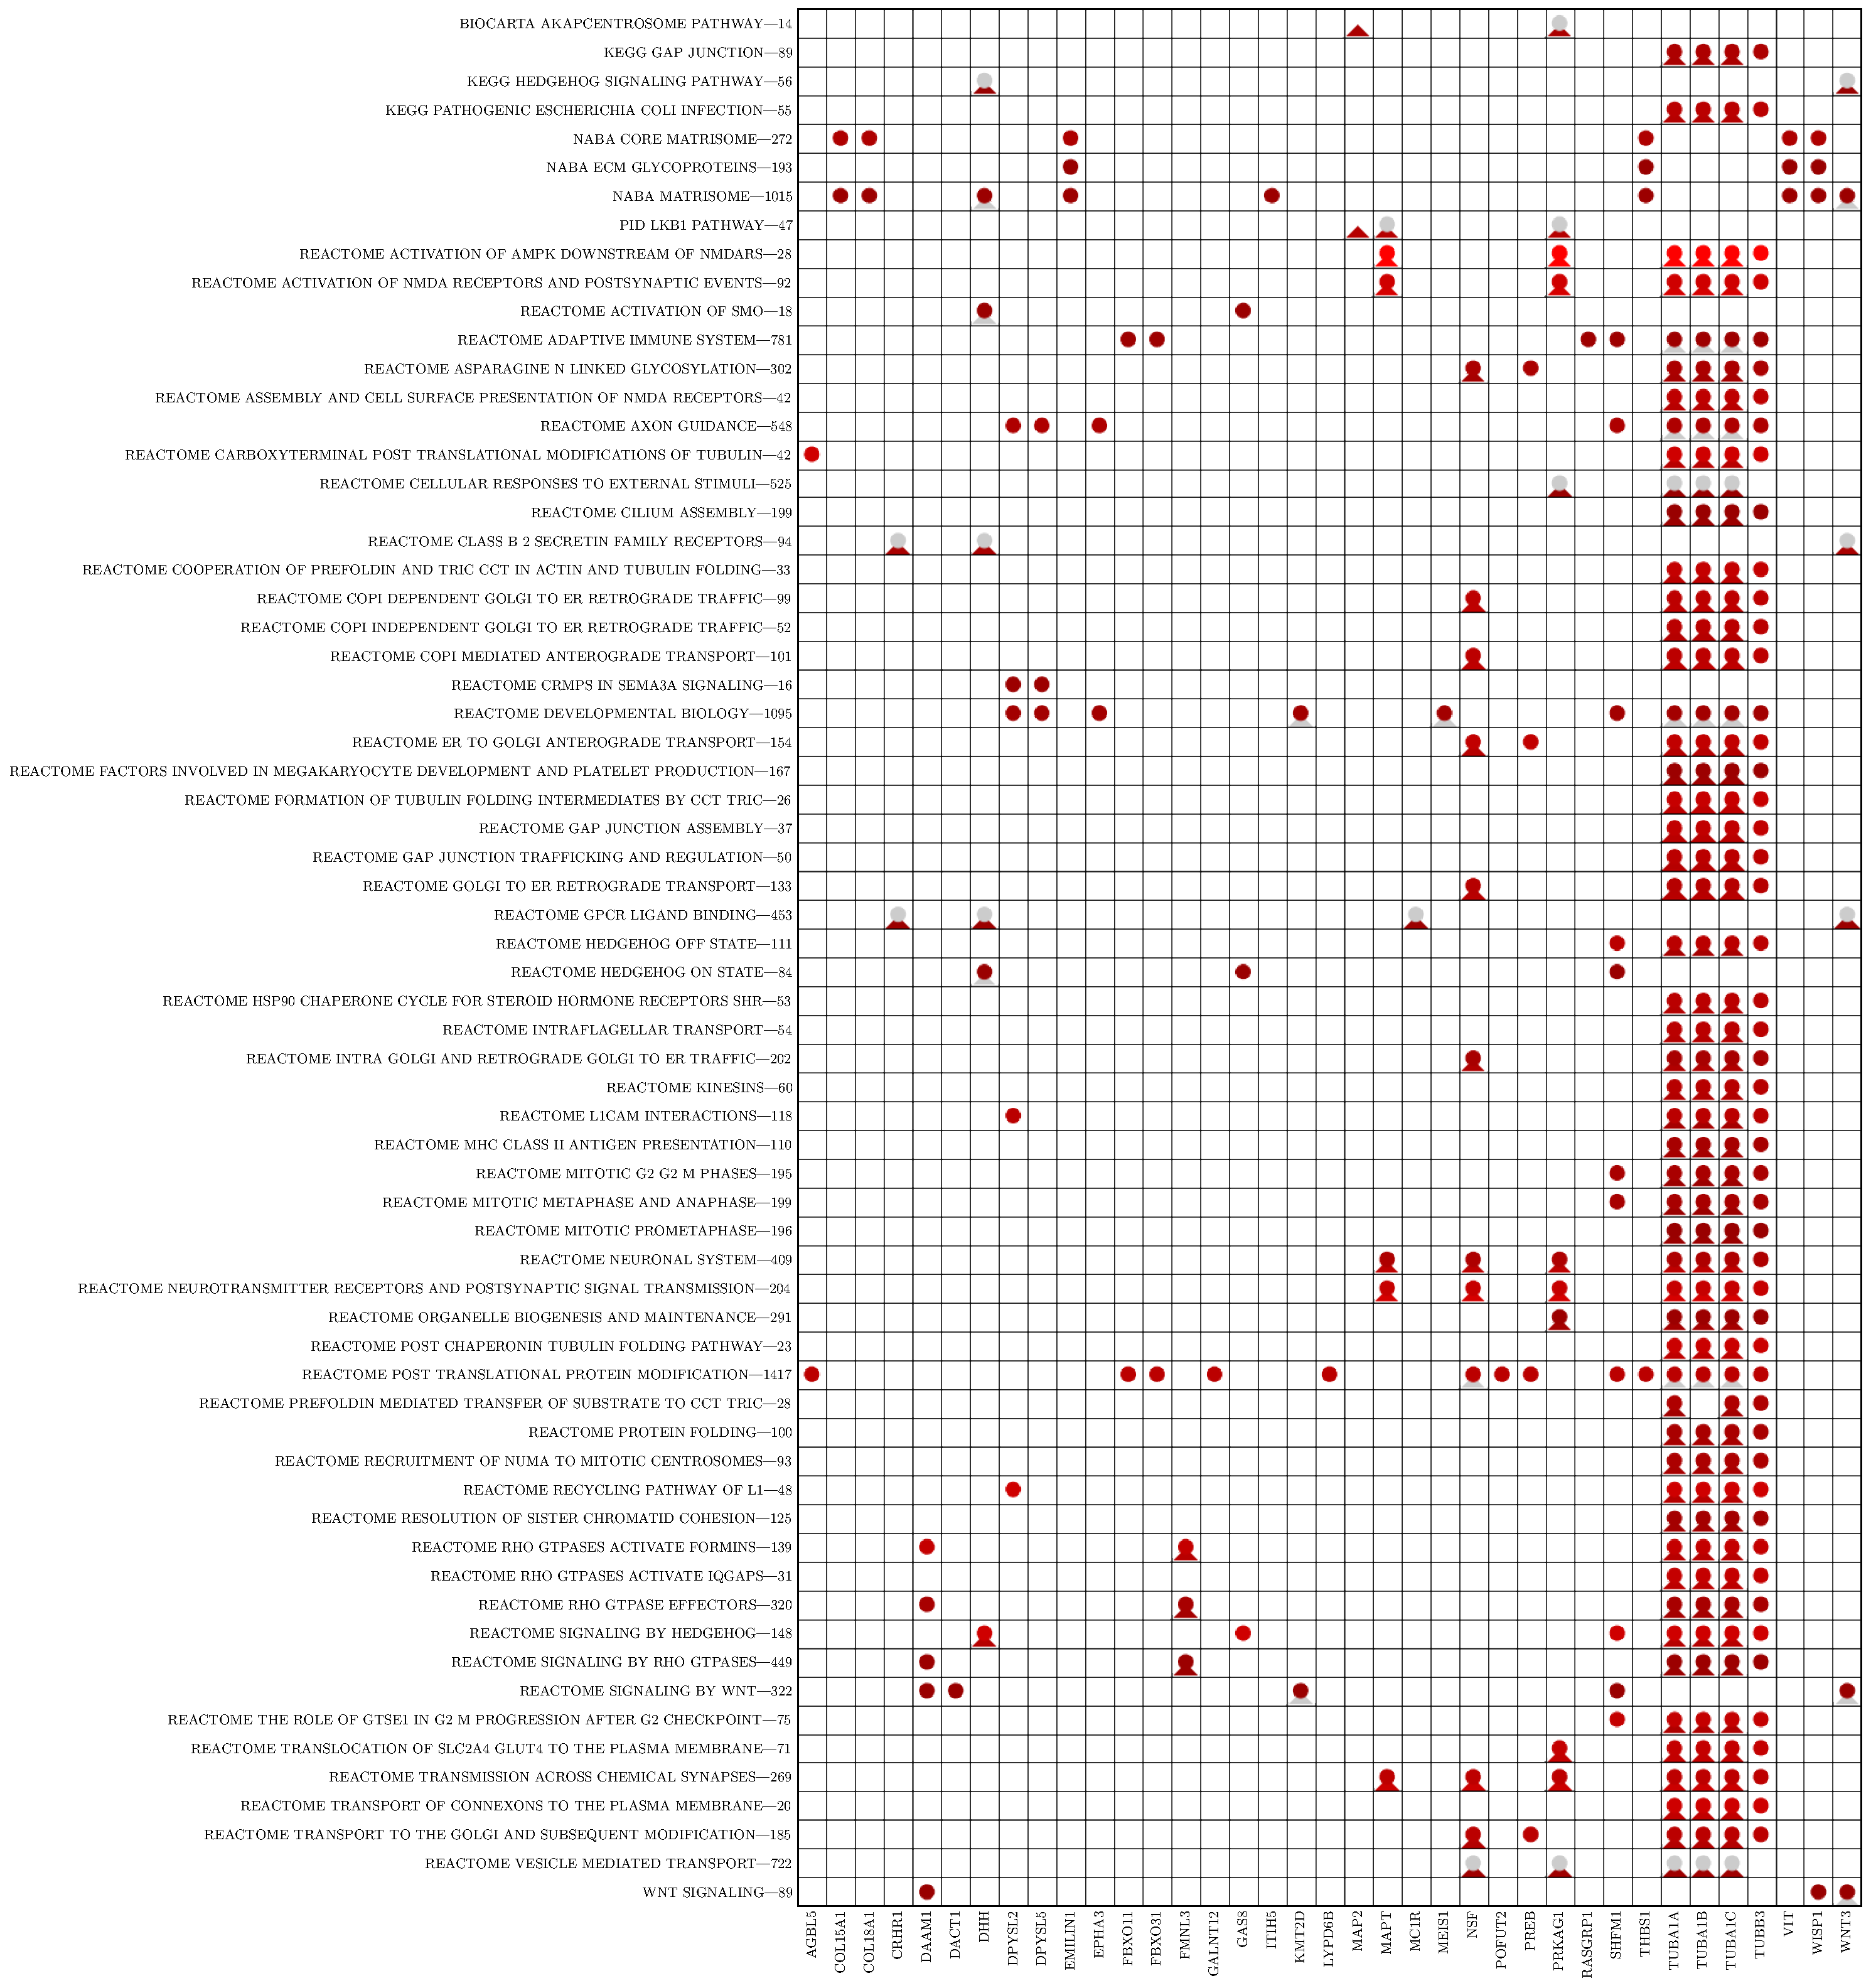
\includegraphics[width=\textwidth]{asymmetry/FUMA gene2func/joinedDatasets/mean_imputed/not_subsampled/partitionsSummary/genes_Canonical_Pathways.pdf}
	
	\caption[Canonical pathways GSEA genes]{Differential gene set enrichment analysis performed on various canonical pathways reported by KEGG and Reactome, as computed by FUMA. Displayed cells have increased lightness the higher the value. The entire hemisphere and the four 2nd level partitions (ie. P1 and P4-P7)) were assessed. With gray, genes are shown that, although intersecting with the trait gene set, were not enough for FUMA to identify significant correlation, based on the underlying gene sets sizes ratios. The partition (P) information per cell is coded as follows: circle: P1, north:P4, east:P5, south:P6, west:P7. Next to the name of the category, the total number of related genes is displayed.}
	\label{fig:can_pathways_genes}
\end{figure}
\end{adjustwidth}
\begin{figure}[H]
	\centering
	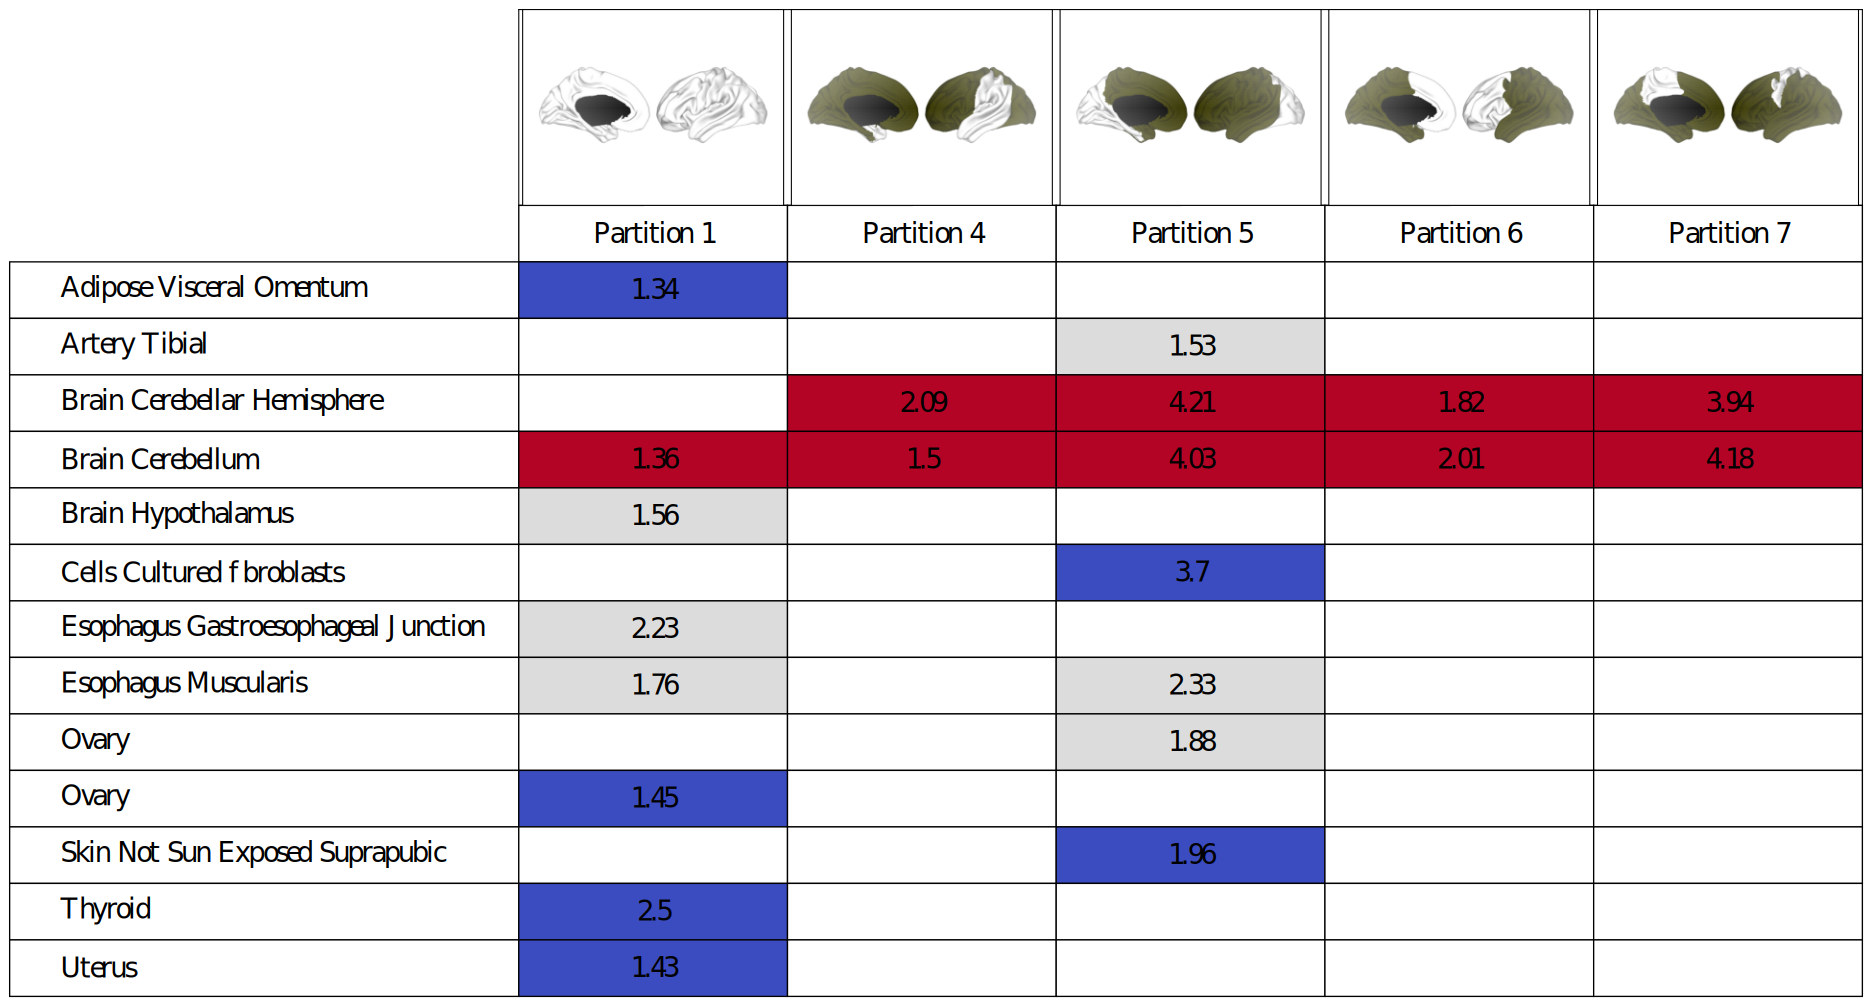
\includegraphics[width=\textwidth]{asymmetry/FUMA gene2func/joinedDatasets/mean_imputed/not_subsampled/partitionsSummary/DEG.pdf}
	
	\caption[Differential gene expression enrichment analysis]{Differential gene expression enrichment analysis performed on different tissues. Displayed -log10 P-values, as computed by FUMA using the identified partition-specific gene sets, are displayed in blue if the relation favors downregulated genes, red if it favors upregulated ones, or gray, if both downregulated and upregulated gene subsets are significantly enriched.}
	\label{fig:de_genes}
\end{figure}
\begin{figure}[H]
	\centering
	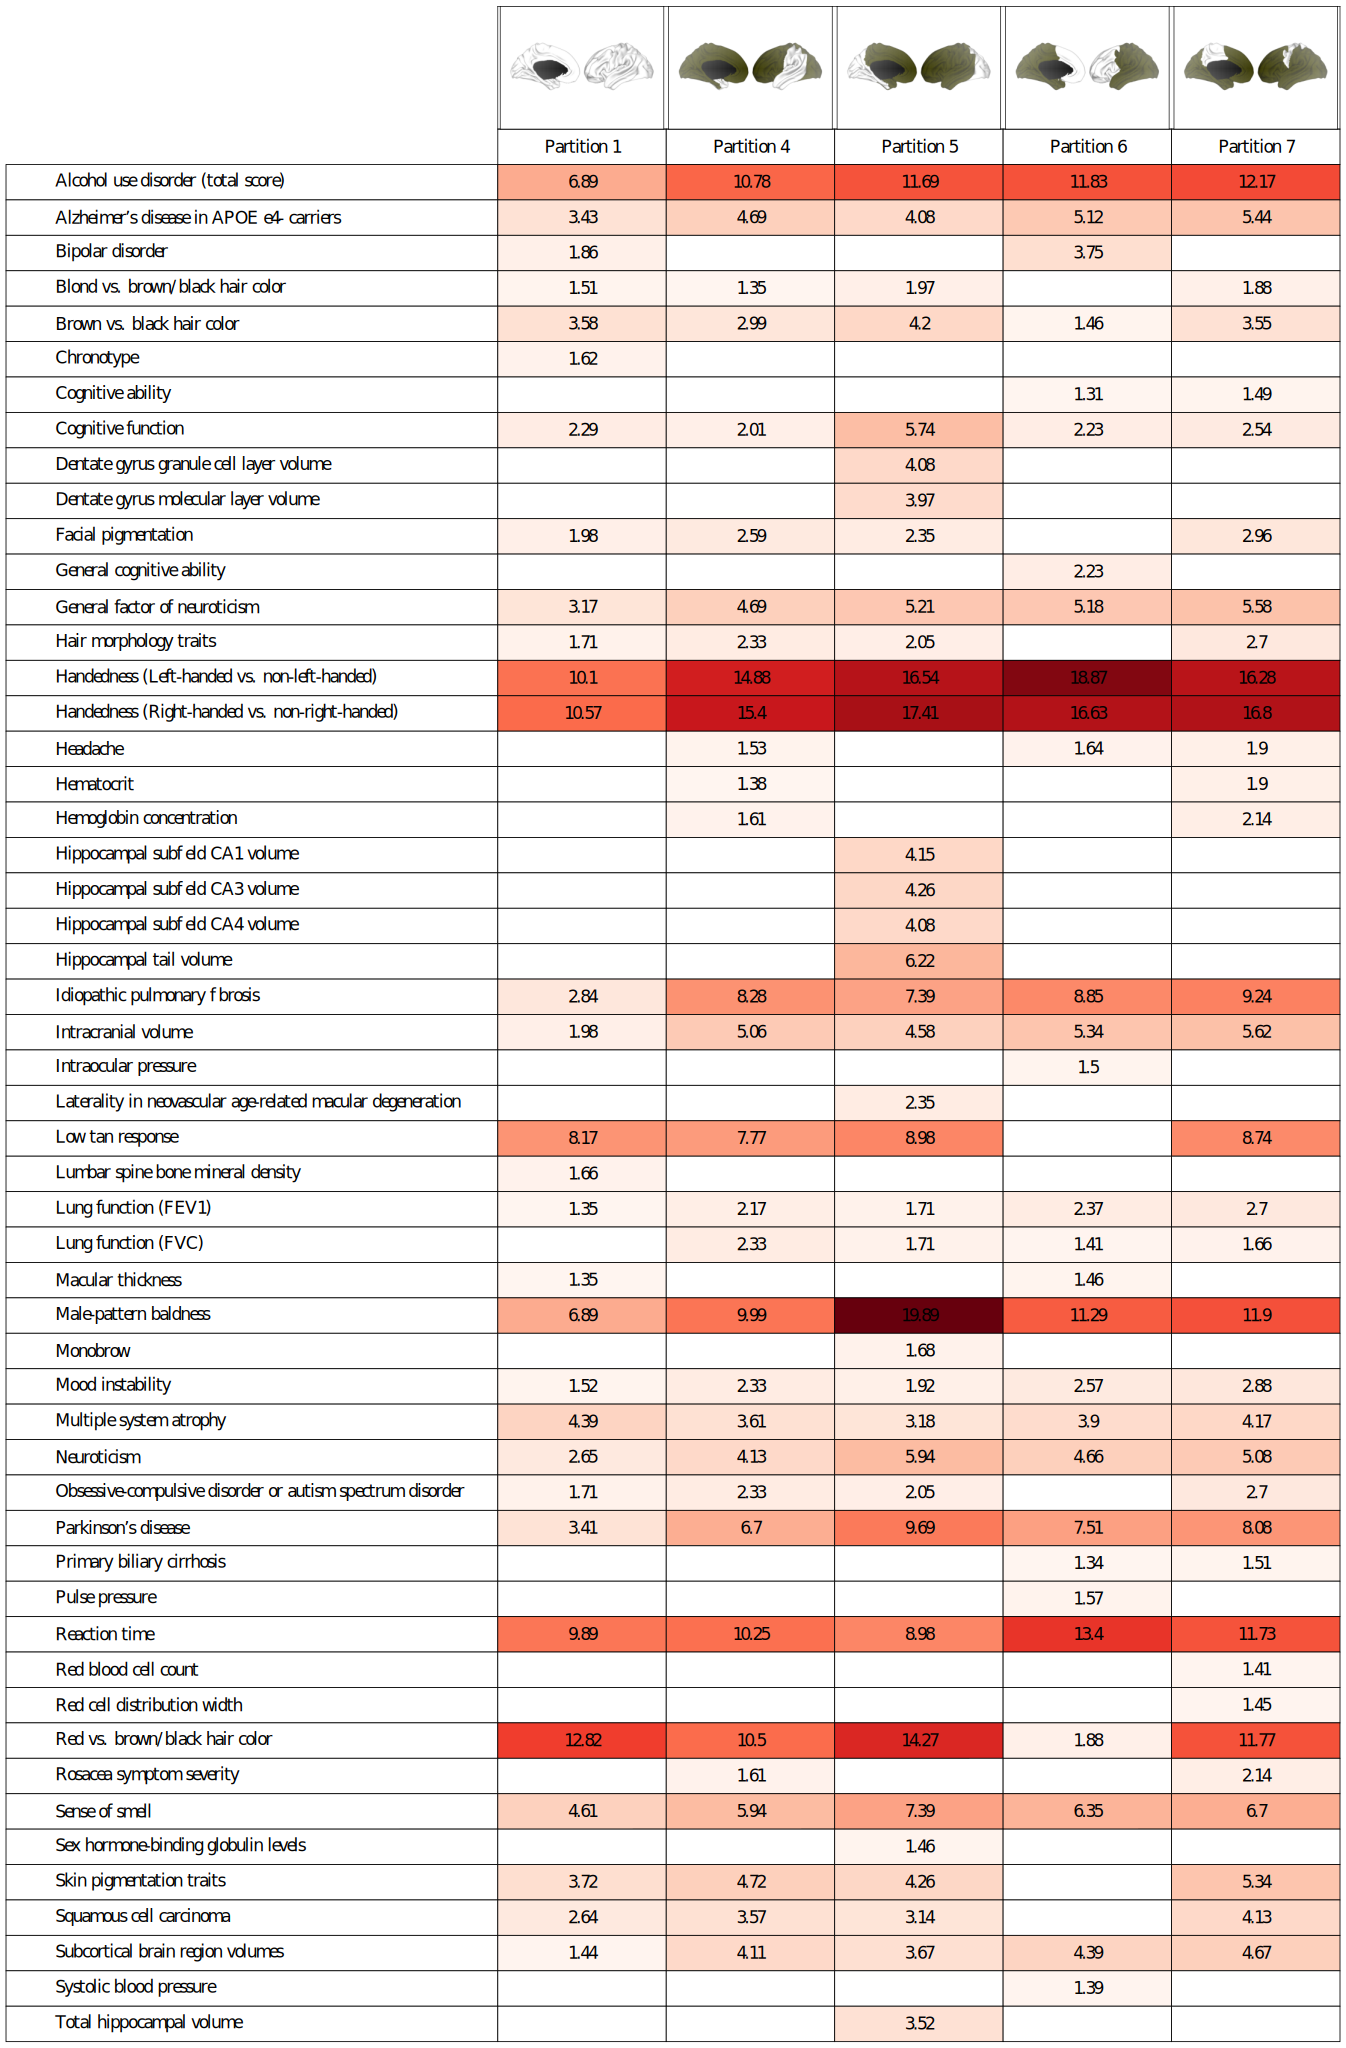
\includegraphics[width=\textwidth]{asymmetry/FUMA gene2func/joinedDatasets/mean_imputed/not_subsampled/partitionsSummary/GWASCatalog.pdf}
	
	\caption[GWAS Catalog GSEA -log10P values]{Differential gene set enrichment analysis performed on various traits reported by GWAS catalog, as computed by FUMA. -log10 P-values are shown, with increased lightness the higher the value.}
	\label{fig:gw_catalog}
\end{figure}
\begin{adjustwidth}{-3cm}{-3cm}
\begin{figure}[H]
	\centering
	\includegraphics[width=\textwidth]{asymmetry/FUMA gene2func/joinedDatasets/mean_imputed/not_subsampled/partitionsSummary/genes_GWASCatalog.pdf}
	
	\caption[GWAS Catalog GSEA genes]{Differential gene set enrichment analysis performed on various traits reported by GWAS catalog, as computed by FUMA. Displayed cells have increased lightness the higher the value. With gray, genes are shown that, although intersecting with the trait gene set, were not enough for FUMA to identify significant correlation, based on the underlying gene sets sizes ratios.  The entire hemisphere and the four 2nd level partitions (ie. P1 and P4-P7)) were assessed. The partition (P) information per cell is coded as follows: circle: P1, north:P4, east:P5, south:P6, west:P7. Next to the name of the category, the total number of related genes is displayed.}
	\label{fig:gw_catalog_genes}
\end{figure}
\end{adjustwidth}